\documentclass[border=4pt]{standalone}
\usepackage[T1]{fontenc}
\usepackage{lmodern}
\usepackage{amsmath,amssymb,bm}
\usepackage{pgfplots}
\pgfplotsset{compat=1.17}
\begin{document}
% Measured on Qwen2.5-0.5B (layers 2-21, 1 chunk, exact share 0, seed 1); see Section 5.
% Theory line: sqrt((n-1)/m) for n = 28 equally sized, mutually orthogonal contributions.
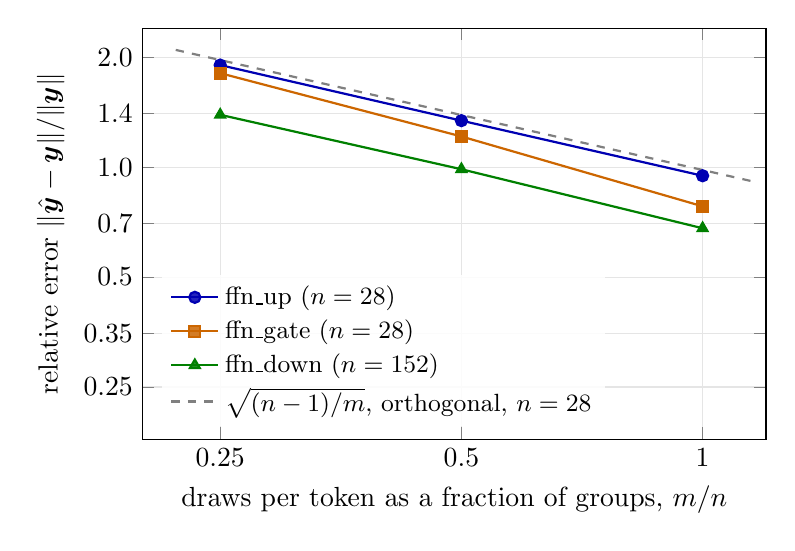
\begin{tikzpicture}
\begin{loglogaxis}[width=9.5cm,height=6.8cm,
    xlabel={draws per token as a fraction of groups, $m/n$},
    ylabel={relative error $\lVert\hat{\bm y}-\bm y\rVert/\lVert \bm y\rVert$},
    xtick={0.25,0.5,1}, xticklabels={0.25,0.5,1},
    ytick={0.25,0.35,0.5,0.7,1,1.4,2}, yticklabels={0.25,0.35,0.5,0.7,1.0,1.4,2.0},
    ymin=0.18, ymax=2.4, xmin=0.2, xmax=1.2,
    legend pos=south west, legend cell align=left, legend style={font=\small,draw=none,fill=white,fill opacity=0.85,text opacity=1},
    grid=major, grid style={gray!20}, every axis plot/.append style={thick}]
  \addplot[blue!70!black,mark=*] coordinates {(0.25,1.902554) (0.5,1.340228) (1.0,0.946842)};
  \addlegendentry{ffn\_up ($n=28$)}
  \addplot[orange!80!black,mark=square*] coordinates {(0.25,1.807966) (0.5,1.212974) (1.0,0.781073)};
  \addlegendentry{ffn\_gate ($n=28$)}
  \addplot[green!50!black,mark=triangle*] coordinates {(0.25,1.390656) (0.5,0.986562) (1.0,0.680082)};
  \addlegendentry{ffn\_down ($n=152$)}
  \addplot[gray,dashed,domain=0.22:1.15,samples=20] {sqrt(27/(28*x))};
  \addlegendentry{$\sqrt{(n-1)/m}$, orthogonal, $n=28$}
\end{loglogaxis}
\end{tikzpicture}
\end{document}
